\documentclass[a4paper]{article}

\usepackage{cmap}
\usepackage[T2A]{fontenc}
\usepackage[utf8]{inputenc}
\usepackage[english,russian]{babel}
\usepackage{amsthm}
\usepackage{amssymb}
\usepackage{amsmath}
\usepackage{mathtools}
\usepackage{indentfirst}
\usepackage{fullpage}
\usepackage{titlesec}
\usepackage{multicol}
\usepackage{parskip}
\usepackage{graphicx}
\usepackage{tikz}
\usepackage{wrapfig}

\newtheoremstyle{definition}{3pt}{3pt}{\upshape}{}{\bfseries}{.}{.5em}{}
\theoremstyle{definition}
\newtheorem{definition}{Опр.}

\newtheoremstyle{statement}{3pt}{3pt}{\upshape}{}{\bfseries}{}{.5em}{}
\theoremstyle{statement}
\newtheorem{statement}{Утв.}
\newtheorem*{statement*}{Утв.}

\newtheoremstyle{note}{3pt}{3pt}{\upshape}{}{\bfseries}{:}{.5em}{}
\theoremstyle{note}
\newtheorem*{note}{Замечание}

\newtheorem{theorem}{Теорема}
\newtheorem*{theorem*}{Теорема}

\newtheoremstyle{example}{3pt}{3pt}{\upshape}{}{\bfseries}{:}{.5em}{}
\theoremstyle{example}
\newtheorem*{example}{Пример}

\title{Лекции по математическому анализу, 3 семестр}
\date{}
\author{Тимошенко Иван, 24123}


\begin{document}
    \maketitle
    \section{Модели комплексных чисел}

\par 
Введем стандартные понятия нужным образом:\\
$\mathbb{R}$ - множество точек на прямой. \\
$\mathbb{C}$ - расширение $\mathbb{R}$ с помощью одного из корней уравнения $z^2 = -1$: $\mathbb{C} = \mathbb{R} \cup  \{0\}$, с замыканием относительно сложения и умножения.

\begin{theorem}[Основная теорема алгебры]
    Множество комплексных чисел ($\mathbb{C}$) алгебраически замкнуто 
    (любой многочлен степени $n$, коэффициенты которого лежат в $\mathbb{C}$),
     имеет корни в $\mathbb{C}$ (с учетом кратности).
\end{theorem}

\begin{note}
    Теорема верна и в частном случае многочлена, определенного над $\mathbb{R}$.
\end{note}

\medskip
\subsection{Стандартная модель комплексных чисел}

Комплексное число $z$ представляется парой $(x, y) \in \mathbb{R}^2$ с операциями:
\begin{itemize}
    \item $"+": \quad (x_1, y_1) + (x_2, y_2) = (x_1+x_2, y_1 + y_2)$
    \item $"\cdot": (x_1, y_1) \cdot (x_2, y_2) = (x_1x_2-y_1y_2, x_2y_1+x_1y_2)$
\end{itemize}

\begin{note}
    Операции согласованы с операциями на $\mathbb{R}.$
\end{note}
\begin{note}
    $\mathbb{R} \subset \mathbb{C}, \quad \mathbb{R} = \{(x, 0) \quad x \in \mathbb{R}\}$
\end{note}
В станд. модели 
$\begin{cases}
    0 = (0, 0)\\
    1 = (1, 0)
\end{cases}$

\begin{definition}
    Мнимая единица определена как пара $(0, 1)$.
\end{definition}
\begin{note}
    Некорректно определять мнимую единицу как корень уравнения $z^2 = -1$, т.к. $-i$ так же является корнем.
    \[i^2 = (0, 1) \cdot (0,1) = (0\cdot0 - 1\cdot1, 0\cdot1 + 1\cdot0) = (-1, 0) = -1\]
    \[(-i^2) = (0, -1)\cdot(0, -1) = (-(-1)\cdot(-1), 0) = (-1, 0) = -1\]
\end{note}
\begin{note}
    Запись $\sqrt{-1}$ тоже некорректна.
\end{note}

\begin{statement}
    На $\mathbb{C}$ нельзя ввести линейный порядок.
    \begin{proof}
        Пусть $x \in \mathbb{C}$, и существует некий линейный порядок <.
        \[\forall x \neq 0
        \begin{cases}
            \text{либо} -\frac{x}{2} < \frac{x}{2} \text{ и } 0 = -\frac{x}{2} + \frac{x}{2} < \frac{x}{2} + \frac{x}{2} = x\\
            \text{либо} \frac{x}{2} < -\frac{x}{2} \text{ и } 0 > x
        \end{cases}
        \]
        Тогда $\forall x \neq 0$ либо $x > 0$, либо $-x > 0$. Т.е. $\forall x \neq 0 \quad x^2 > 0$.
        Но $-1 = i^2 < 0$ - противоречие.
    \end{proof}
\end{statement}

\bigskip

\subsection{Матричная модель}
Комплексное число $z = \begin{pmatrix}
    x & y\\
    -y & x
\end{pmatrix}$, где $x, y \in \mathbb{R}$.

\["+": 
    \begin{pmatrix}
        x_1 & y_1 \\
        -y_1 & x_1
    \end{pmatrix} 
    + 
    \begin{pmatrix}
        x_2 & y_2 \\
        -y_2 & x_2 \\
    \end{pmatrix}
    =
    \begin{pmatrix}
        x_1 + x_2 & y_1 + y_2 \\
        -y_1 - y_2 & x_1 + x_2
    \end{pmatrix}
\]
\["\cdot": 
    \begin{pmatrix}
        x_1 & y_1 \\
        -y_1 & x_1
    \end{pmatrix} 
    \cdot
    \begin{pmatrix}
        x_2 & y_2 \\
        -y_2 & x_2 \\
    \end{pmatrix}
    =
    \begin{pmatrix}
        x_1x_2 - y_1y_2 & x_1y_2 + x_2y_1 \\
        -x_1y_2 - x_2y_1 & x_1x_2 - y_1y_2
    \end{pmatrix}
\]

В матричной модели ноль (нейтральный элемент по сложению) представлен матрицей
$0 =\begin{pmatrix}
    0 & 0 \\
    0 & 0
\end{pmatrix}$, единица (нейтральный по умножению)
$1 = \begin{pmatrix}
    1 & 0 \\
    0 & 1
\end{pmatrix}$, мнимая единица  
$i = \begin{pmatrix}
    0 & 1 \\
    -1 & 0
\end{pmatrix}$.

В стандартной модели произвольное комплексное число $z = (x, y)$ 
имеет стандартную запись \\$z = x + iy$, где $\begin{cases}
    x - \text{вещественная часть}\\
    y = \text{мнимая часть}
\end{cases}$

Действия с комплексными числами:
\begin{enumerate}
    \item Сравнение (проверка равенства):
        \[a + ib = c + id \iff a = c \text{ и } b = d\].
    \item Сложение:
        \[(a+ib) + (c+id) = (a+c) + i(b+d)\]
    \item Умножение:
        \[(a+ib)\cdot(c+id) = (ac - bd) + i (ad + bc)\]
    \item Деление:
        \[\frac{a+ib}{c+id} = \frac{(a+ib)\cdot(c-id)}{c^2+d^2} = \frac{(ac - bd) + i(bc - ad)}{c^2 + d^2}\]
\end{enumerate}


\subsection{Геометрическая модель}

Комплексное число представлено точкой с координатами $(x, y)$ на плоскости.\\
Операции:
\begin{itemize}
    \item $"+"$: действует как сложение векторов (покоординатно).
    \item $"\cdot": z_3 = z_1z_2 \iff \begin{cases}
        |z_3| = |z_1|\cdot|z_2| \\
        arg(z_3) = arg(z_1) + arg(z_2)
    \end{cases}$
    \\ где $|z| = \sqrt{x^2 + y^2}, \quad arg(z)$ задает угол между $\vec{z}$ и Ox 
    (определяется с точностью до периода).
\end{itemize}

\textbf{Аргумент комплексного числа} $Arg(z)$ - угол $\varphi$ c точностью до периода $2\pi$.
\textbf{Главное значение аргумента} $arg(z)$ - $\varphi$  в промежутке $[0; 2\pi]$.

\textbf{Комплексно сопряженное к} $z = x+iy$ это $\overline{z} = x - iy$.
\[|z| = |\overline{z}|, \quad arg(z) = -arg(\overline{z}), \quad 
Re(z) = Re(\overline{z}), \quad Im(z) = -Im(\overline{z})\] 
\[\overline{z} \cdot z = (x+iy)\cdot(x-iy) = x^2 + y^2 = |z|^2\] 

\textbf{Законы де Моргана:}
\begin{itemize}
    \item $\overline{(\overline{z})} = z$
    \item $\overline{z_1 + z_2} = \overline{z_1} + \overline{z_2}$
    \item $\overline{z_1z_2} = \overline{z_1} \cdot \overline{z_2}$
\end{itemize}

\textbf{Неравенство треугольника:}
\[\begin{cases}
    |z_1 + z_2| \leq |z_1| + |z_2|\\
    |z_1 - z_2| \geq \lvert \lvert z_1\rvert - \lvert z_2\rvert \rvert
\end{cases} \implies \lvert \lvert z_1 \rvert - \lvert z_2 \rvert \rvert \leq 
\lvert z_1 + z_2 \rvert \leq \lvert z_1 \rvert + \lvert z_2 \rvert \]

\subsection{Стереографическая проекция}
На комплексную плоскость положили сферу $S$ радиуса $\frac{1}{2}$. Северный полюс сферы - вершина $N(0; 0; 1)$.
Комплексному числу $c$, лежащему в плоскости комплексных чисел и имеющему координаты $(x, y, 0)$ ставится в соответствие точка, которая является точкой пересечения прямой $Nc$ со сферой $S$. 
Зададим систему координат $O\xi \eta \zeta$ аналогично $Oxyz$, 
но $O$ имеет координаты $(0, 0, \frac{1}{2})$.\\
Уравнение сферы S:
\begin{equation} 
    \label{RimanSphereEq}
    \xi^2 + \eta^2 + (\xi - \frac{1}{2})^2 = (\frac{1}{2})^2
\end{equation}
Уравнение прямой $Nc$ по двум точкам:
\begin{equation}
    \label{NcEq}
    \frac{\xi}{x} = \frac{\eta}{y}=\frac{\zeta-1}{-1} 
    \iff
    \xi^2 + \eta^2 + \zeta^2 - \zeta = 0
\end{equation}

Получаем набор \textbf{обратных формул стереографической проекции:}
$x = \frac{\xi}{1 - \zeta}, y = \frac{\eta}{1-\zeta}, z = \frac{\xi + i\eta}{\zeta - 1}$.
Отсюда найдем
\begin{equation}
    \label{zsphere}
    \left| z \right|^2 = z \cdot \overline{z} = \frac{\xi^2 + \eta^2}{(1-\zeta)^2}
    \underset{\text{из } \ref{NcEq}}{=} \frac{\zeta}{1-\zeta} 
    \implies \zeta = \frac{\left| z \right|^2}{1 + \left| z\right|^2}
\end{equation}
Подставим \ref{zsphere} в уравнение \ref{RimanSphereEq} и получим прямые формулы стереографической проекции:
\begin{equation}
    \xi = \frac{x}{1 + \left|z\right|^2}, \quad
    \eta = \frac{y}{1 + \left|z\right|^2}, \quad
    \zeta = \frac{\left|z\right|^2}{1 + \left|z\right|^2}
\end{equation}

Из геометр. постреония стереографическая проекция взаимно однозначно 
отображает комплексную плокость на сферу $S \setminus \{N\}$.
Дополним стер. проекцию по непрерывности:
\begin{equation}
    P: \overline{\mathbb{C}} \overset{\text{на}}{\to}S \quad
    \text{где } \overline{\mathbb{C}} = \mathbb{C} \cup \{\infty\}, \text{а $S$ называют сферой Римана.}
\end{equation}

\begin{definition}
    Обобщенная окрестность на комплексной плоскости - это любая окружность (или прямая, рассмотренная как окружность бесконечного радиуса).
\end{definition}

Свойства стереографической проекции:
\begin{enumerate}
    \item Для любой обобщенной окружности $l \subset \overline{\mathbb{C}}$ ее образ $P(l) \subset S^2$ - это окружность.
    \begin{proof}
        Пусть $l$ - некая обобщ. окрестность на $\overline{\mathbb{C}}$, тогда ее уравнение:
        \[l: A(x^2+y^2) + Bx + Cy + D = 0 \text{ - окружность при $A \neq 0$, прямая при $A = 0$}\]
        Подставим в него обратные формулы стереогр. проекции:
        \begin{equation}
            A\frac{\zeta}{1 - \zeta} + B\frac{\xi}{1 - \zeta} + C\frac{\eta}{1 - \zeta} + D = 0
        \end{equation}
        Поделим на $1 - \zeta$ и получим:
        \begin{equation}
            \label{FlatEq}
            \text{П: }B\xi + C\eta + (A-D)\zeta + D = 0
        \end{equation}
        Но это уравнение некоторой плоскости П в $\mathbb{R}^3$, кроме того, $P(l) \subset S^2$,
        значит для $l$ выполнено уравнение сферы Римана $\xi^2 + \eta^2 + \zeta^2 - \zeta = 0$.
        Тогда $P(l) = S^2 \cap \text{П}$ - пересечение сферы с плоскосью окружность.
    \end{proof}

    \item $\forall$ окружности $L \subset S^2 \ P^{-1}(L)$ является обобщенной окружностью на $\overline{\mathbb{C}}$.
    \begin{proof}
        Плоскость $\Pi \subset \mathbb{R}^3$ такая, что $\Pi \cap S^2 = L$,
        а значит ее уравнение имеет \\ вид (\ref{FlatEq}). Разделим (\ref{FlatEq}) на $1-\zeta$, получим обобщенное уравнение прямой,
        подставим туда прямые формулы проекции и получим уравнение вида $A(x^2+y^2)+Bx +Cy + D = 0$, а это - уравнение обобщенной окружности в $\overline{\mathbb{C}}$.
    \end{proof}

    \item Стереографическая проекция сохраняет углы. То есть $\forall l_1, l_2 \in \overline{\mathbb{C}} \text{ таких, что } l_1 \cap l_2 \neq \empty$
    и $\alpha$ - угол между ними, верно, что угол между $P(l_1)$ и $P(l_2)$ тоже равен $\alpha$ (угол между окружностями это угол
    между касательными в точке пересечения).
\end{enumerate}

\begin{definition}
    Кривая - это функция (или ее образ) $g: [a, b] \to \mathbb{R}^2$. Параметром кривой $g$ называют $t \in [a, b]$. 
    \[\overrightarrow{v} = \frac{\frac{\partial \overrightarrow{g}}{\partial t}}{\left| \frac{\partial g}{\partial t}\right|} = \left( \frac{\frac{\partial x}{\partial t}}{\left| \frac{\partial g}{\partial t}\right|}, \ \frac{\frac{\partial y}{\partial t}}{\left| \frac{\partial g}{\partial t}\right|} \right) \quad \overrightarrow{n} = \frac{\frac{\partial^2 g}{\partial t^2}}{\left| \frac{\partial^2 g}{\partial t^2} \right|}\]
    Натуральный параметр на кривой $g$ это $l \subset [0, L]$ ($L$ - длина $g$), такой, что $\forall l$ выполнено $\frac{\partial g}{\partial l} = 1$.
    Набор $\{v, n\}$ называется базис Френе, для него выполена теорема Френе. 
    Уравнения Френе:
    \[
    \frac{d}{dl} \begin{pmatrix} v \\ n \end{pmatrix} = 
    \begin{pmatrix}
        0 & k(l) \\
        -k(l) & 0
    \end{pmatrix}
    \begin{pmatrix} v \\ n \end{pmatrix}, \quad k(l) \text{ называется кривизной } g \subset \mathbb{R}^2
    \]
\end{definition}

\subsection{Виды записи}
Стандартная запись $z = x + iy$. \\
Пусть $r = \left| z \right|, \ \varphi = arg(z)$.
\begin{definition}
    Тригонометрическая запись комплексного числа:
    \[\begin{cases}
        Re(z) = x = r\cdot \cos(\varphi) \\ 
        Im(z) = y = r\cdot \sin(\varphi)
    \end{cases} \implies z = x +iy = r(\cos(\varphi) + i\sin(\varphi))\]
\end{definition}
    
\begin{definition}
    Формула Эйлера:
    \[e^{i\varphi} = \cos(\varphi) + i\sin(\varphi) \implies z = re^{i\varphi}\]
    Тогда для натурального $n$:
    \[z^n = r^n e^{in\varphi} = r^n (\cos(n\varphi) + i\sin(n\varphi))\]
    Пусть $z \neq 0 \implies r = \left| z \right| > 0$. тогда $z^{\frac{1}{n}} = r^{\frac{1}{n}}\cdot e^{\frac{i(\varphi + 2\pi k)}{n}}$, где $k = 0 \hdots n-1$.
    Отсюда же получается формула Муавра для корней степени $n$ из $z \neq 0$:
    \[z^{\frac{1}{n}} = r^{\frac{1}{n}}(\cos(\frac{\varphi + 2\pi k}{n})+ i\sin(\frac{\varphi + 2\pi k}{n}))\]
\end{definition}

\begin{note}
    $\exists n$ различных корней степени $n$ из комплексного числа $z \neq 0$.
    \[z_0, z_1, \hdots z_{n-1} \in \text{ окружности радиуса } r^{\frac{1}{n}} \text{ c центром в } (0,0)\]
\end{note}

    \begin{definition}
    Функция дифференциируема в точке, если 
    \begin{itemize}
        \item $f:U \to \mathbb{R}^k$ и $p \in Int(U)$
        \item $f(x) = f(p) + df(p)\langle x-p \rangle + \alpha(x),$ где $\alpha(x) = o(x-p).$
    \end{itemize}
\end{definition}
Если $k = 1$, то лин. отображение $df(p):\mathbb{R}^n \to \mathbb{R}$
можно задатьа как $df(p)\langle v \rangle = \langle \nabla f(p);  v \rangle$
 - скалярное произведение градиента функции на вектор, причем 
 $\nabla f(p) = \left(\frac{\partial f}{\partial x_1}(p), \dots, \frac{\partial f}{\partial x_n}(p)\right)$ - вектор частных производных в точке $p$.

\begin{statement}
    Градиент функции задает направление, при движении в котором функция растет быстрее всего.
    \begin{proof}
        Рассмотрим функцию $f$ в точке $p$, вектор $v$ единичной длины будет задавать произвольное направление.
        \begin{equation*}\frac{f(p+tv) - f(p)}{t} \underset{t \to 0}{\to}
            \frac{\partial f}{\partial v} = df(p)\langle v \rangle = \langle \nabla f(p); v \rangle 
            = |\nabla f(p)| \cdot |v| \cdot cos(\varphi), \text{где $\varphi $ - угол между $\nabla f$ и $v$.}
        \end{equation*}
        Поскольку $|\nabla f(p) = const, |v| = 1$, то для максимизации надо выбрать такое $\varphi$, 
        чтобы $cos(varphi)$ был максимален, т.е. вектора $v$ и $\nabla f$ параллельны и $\nabla f$ задает наибольшую скорость роста.
    \end{proof}
\end{statement}

\begin{statement}
    $\nabla f(p)$ ортогонален поверхности уровня $\Omega = \{x | f(x) = c\}$.
    \begin{proof}
        Пусть $f(p) = c \ (p \in \Omega)$. Пусть $x_n \in \Omega$, покажем, что $cos(\nabla f(p), \overrightarrow{x_n-p}) \underset{n \to \infty}{\to} 0:$
        \begin{eqnarray*}
            f(x_n) = f(p) = c \implies 0 = f(x_n) - f(p) = df(p)\langle x_n-p \rangle + o(x_n - p) = 
            \langle \nabla f(p); x_n - p \rangle + o(x_n - p).
        \end{eqnarray*}
        Значит $0 \underset{n \to \infty}{=} \langle \nabla f(p); \frac{x_n - p}{|x_n - p|} \rangle + o(1)$, т.е.
        $\langle \nabla f(p); \frac{x_n - p}{|x_n - p|} \rangle \to 0 $. Тогда:
        \begin{equation*}
            \langle \nabla f(p); \frac{x_n - p}{|x_n - p|} \rangle = |\nabla f(p)|\cdot \left|\frac{x_n-p}{|x_n-p|}\right|\cdot cos(\alpha) \to 0, 
            \ \text{т.е.} \alpha \underset{n \to \infty}{\to} \frac{\pi}{2}. 
        \end{equation*}
        
    \end{proof}
\end{statement}

\begin{definition}
    Функция $f:\mathbb{R}^n \to \mathbb{R}^n$ называется векторным полем.
\end{definition}
\begin{definition}
    Потенциалом векторного поля $F$ (если он есть) называется \textbf{скалярная} функция $U:W \to \mathbb{R}$, 
    такая, что $\nabla U = F$. Если потенциал существует, то F называется потенциальным полем.

\end{definition}

\begin{theorem*}
    Пусть $f:U \subset \mathbb{R}^n \to \mathbb{R}^k, \ g:V \subset \mathbb{R}^k \to \mathbb{R}^m, \ f \in C^1(p), \ g \in C^1(q), \ q = f(p)$.\\
    Тогда $g \circ f \in C^1(p), \, dg \circ f = dg(f(p)) \cdot df(p).$ В матрицах Якоби: $D_{g \circ f}(p) = D_g(f(p)) \cdot D_f(p).$
\end{theorem*}

\begin{example}
    \begin{equation*}
        \begin{cases}
            f(x, y, z) = (xy, xz): \mathbb{R}^3 \to \mathbb{R}^2\\
            g(a, b) = \cosh(ab): \mathbb{R}^2 \to \mathbb{R}
        \end{cases} \quad
        f =
        \begin{cases}
            f_1(x, y, z) = xy\\
            f_2(x, y, z) = xz.
        \end{cases}
    \end{equation*}

    \begin{equation*}
        h = g(f(x, y, z)) = \cosh(xy \cdot xz): \mbox{R}^3 \to \mathbb{R}, \quad (x, y, z) \in \mathbb{R}^3 \overset{f}{\to} \mathbb{R}^3 \overset{g}{\to} \mathbb{R}
    \end{equation*}
    \begin{equation*}
        \frac{\partial h}{\partial x} = \sinh(x^2yz)\cdot 2xyz \quad
        \frac{\partial h}{\partial y} = \sinh(x^2yz)\cdot x^2z \quad
        \frac{\partial h}{\partial z} = \sinh(x^2yz) \cdot x^2y
    \end{equation*}

    \[D_f(x, y, z) = \begin{pmatrix}
        \frac{\partial f_1}{\partial x} & \frac{\partial f_1}{\partial y} &  \frac{\partial f_1}{\partial z} \\
        \frac{\partial f_2}{\partial x} & \frac{\partial f_2}{\partial y} &  \frac{\partial f_2}{\partial z}  
    \end{pmatrix} =
    \begin{pmatrix}
        y & x & 0 \\
        z & 0 & x
    \end{pmatrix}
    \]

    \[D_f = \begin{pmatrix}
        \sinh(ab)\cdot a & \sinh(ab) \cdot b
    \end{pmatrix}\]

    \[D_g \cdot D_f = \begin{pmatrix}
        \sinh(x^2yz)\cdot xz & \sinh(x^2yz)\cdot xy
    \end{pmatrix} \cdot \begin{pmatrix}
        y & x & 0 \\
        z & 0 & x
    \end{pmatrix}
    \]
    Досчитывать я это не буду, поверим Сторожуку на слово.
\end{example}

\textbf{Правило дифференциирования обратного отображения:}
Если невырождено и $\exists$ обратное отображение $g:V \to U$, непрерывное в точке $q = f(p)$, тогда:
\[g \in D(q) \text{ и } dg(q) = (df(p))^{-1}\]


\subsection{Многократная дифференциируемость}

\begin{definition}
    $f: U \subset \mathbb{R}^n \to \mathbb{R}^m \ k$ раз дифференциируема в точке $p$ ($f \in D^k(p)$), если:
    \begin{enumerate}
        \item $f$ дифференциируема во всех точках некоторой окрестности точки $p$;
        \item Все частные производные $\frac{\partial f}{\partial x_1}, \dots, \frac{\partial f}{\partial x_n}$ дифференциируемы $k-1$ раз в точке $p$.
    \end{enumerate}  
\end{definition}

\begin{example}
    \[f \in D^2(p) \implies f \in D(x) \text{ и } \frac{\partial f}{\partial x}, \frac{\partial f}{\partial y} \in D(p)  \]
\end{example}

\begin{statement*}
    Если $\begin{cases}
        f \in D^k(p): \mathbb{R}^n \to \mathbb{R}^k\\
        g \in D^k(p): \mathbb{R}^n \to \mathbb{R}^k
    \end{cases}$ тогда $h(x) = f(x) \cdot g(x) \in D^k(p)$

    \begin{proof}
        \begin{equation*}
            \frac{\partial h}{\partial x_i}(x) = \frac{\partial f}{\partial x_i}(x)\cdot g(x) +
            f(x) \cdot \frac{\partial g}{\partial x_i}
        \end{equation*}
        Так как $\frac{\partial f}{\partial x_i}(x) \in D^{k-1}(p), \ g(x) \in D^k(p), \ f(x) \in D^k(p), \ \frac{\partial g}{\partial x_i} \in D^{k-1}(p)$,
        то $\frac{\partial h}{\partial x_i} \in D^{k-1}(p)$.
    \end{proof}
\end{statement*}


\begin{theorem}[о вторых производных]
    Пусть $f:U \subset \mathbb{R}^n \to \mathbb{R}, \ f \in D^2(p)$. Тогда $\frac{\partial^2 f}{\partial x \partial y} = \frac{\partial^2 g}{\partial y \partial x}$.
    \begin{proof}
        Можно считать, что $n = 2$, так как при заданной функции $f(x_1, x_2, \dots)$ можно в качестве $f$ рассмотреть 
        сужение $f$ на плоскость $Ox_1x_2$, т.к. при дифференциировании по $x_1$ или $x_2$ остальные переменные не изменются.

        \[f = f(x, y) \in D^2(p), \quad p = (x_0, y_0, \dots)\]
        Считаем, что $p = 0$ и что $\frac{\partial f}{\partial x}(0) = 0, \ \frac{\partial f}{\partial y}(0) = 0$.
        Чтобы показать почему так можно считать введем $f_1$:
        \[f_1(x, y) := f(x,y) - f'_x(0, 0)\cdot x - f'_y(0,0)\cdot y\]
        \[\frac{\partial f_1}{\partial x}(0, 0) = \frac{\partial f}{\partial x}(0, 0) - f'_x(0,0)\]
        \[\frac{\partial f_1}{\partial y}(0,0) = \frac{\partial f}{\partial y}(0,0) - f'_y(0,0)\]
        
        Дальше считаем, что $f = f_1$ и $f(0,0) = 0$. 
        \begin{equation*}
            \frac{\partial f}{\partial x }(x, y) =f(0,0) + a_{11}\cdot x + a_{12}\cdot y + \alpha_1(x, y), \ \text{где }
            \alpha_1(x, y) = o(x, y), \ (a_{11}, a_{12}) = df(0,0)\langle x, y \rangle
        \end{equation*}
        По условию $\frac{\partial f}{\partial x}, \frac{\partial f}{\partial y} \in D(0)$, поэтому 
        $a_{11} = f_{xx}(0), \ a_{12} = f_{xy}(0)$.
        \[\frac{\partial f}{\partial y}(x, y) = f(0,0) + a_{21}\cdot x + a_{22}\cdot y + \alpha_2(x, y), \ 
        a_{21} = f_{yx}(0), \ a_{22} = f_{yy}(0)\]

        \newpage
        \begin{minipage}[t]{0.45\textwidth}        
            \begin{tikzpicture}[remember picture, overlay]
                \node[anchor=north west, yshift=5pt, xshift=10pt] at (current page.north west) {
                    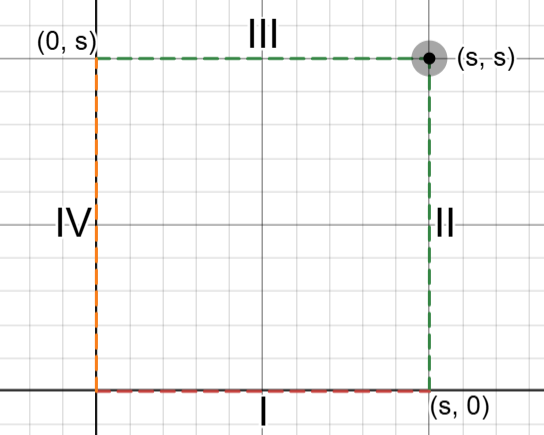
\includegraphics{График_для_теоремы_Шварца.png}
                };
            \end{tikzpicture}
        \end{minipage}
        \begin{minipage}[t]{0.5\textwidth}
            Рассмотрим точку $(s,s)$ вблизи нуля. Для нее 
            $f(s,s) - f(0,0) = (f(s,s) - f(s, 0)) + (f(s,0) - f(0,0)) = (II) + (I)$. \newline
            И в то же время $f(s, s) =  (\text{IV}) + (\text{III})$
        \end{minipage}
        \\[100pt]
        \[\text{II} = f(s,s) - f(s,0) = \int_{y=0}^{s}\frac{\partial f}{\partial y}(s,t)dt
        = \int_{t=0}^{s}a_{21}s + a_{22}t + \alpha_2(s,t)dt = a_{21}s^2 + \frac{a_{22}s^2}{2} + \varepsilon_1(s),\]
        причем $\varepsilon_1(s) = \int_{t=0}^{s}\alpha_2(s,t)dt$. Аналогично для I:
        \[\text{I} = f(s,0) - f(0,0) = \int_{t=0}^{s}\frac{\partial f}{\partial x}(t,0)dt = \int_{t=0}^{s}a_{11}t+a_{12}\cdot0 + \alpha_1(t)dt = 
        \frac{a_{11}}{2}s^2 + \varepsilon_2(s), \ \varepsilon_2(s) = \int_{t=0}^{s}\alpha_1(t,0)dt\]
        
        Итого: $f(s,s) - f(0,0) = \text{I} + \text{II} = s^2 \left( a_{21} + \frac{a_{11}}{2} + \frac{a_{22}}{2}+ \frac{\varepsilon_1(s) + \varepsilon_2(s)}{s^2}\right)$, что на самом деле равно $\text{III} + \text{IV} = 
        \\ = s^2\left(a_{12} + \frac{a_{11}}{2} + \frac{a_{22}}{2} + \frac{\varepsilon_3(s) + \varepsilon_4(s)}{s^2}\right)$
        
    
    \end{proof}
\end{theorem}
\end{document}